\chapter{Bab 1}

\section{Variabel}

Menurut dari tata letak penempatan deklarasi, variabel dibagi menjadi 3. yaitu:\\
1. Variabel Global\\
Variabel Global adalah variabel yang dideklarasikan di luar fungsi. artinya variabel global dapat diakses di dalam atau di luar fungsi.\\

x = "global"\\

def foo():\\
    print("x inside :", x)\\

foo()\\
print("x outside:\\

penjelasan :\\
x sebagai variabel global dan mendefinisikan a foo()untuk mencetak variabel global x . Akhirnya, kami memanggil foo() yang akan mencetak nilai x .

2. Variabel Lokal\\
Variabel Lokal adalah Variabel yang dideklarasikan di dalam tubuh fungsi. artinya variabel hanya dapat diakses di dalam fungsi.\\

def foo():\\
    y = "local"\\
    print(y)\\

foo()\\

penjelasan :\\
variabel lokal y dalam lingkup global dan variabel lokal hanya berfungsi di dalam  foo()

3. Variabel Non Lokal\\
Variabel non lokal digunakan dalam fungsi bersarang yang cakupan lokalnya tidak ditentukan. Ini berarti, variabelnya tidak bisa dalam lingkup lokal maupun global.\\

def outer():\\
    x = "local"\\
    
    def inner():\\
        nonlocal x\\
        x = "nonlocal"\\
        print("inner:", x)\\
    
    inner()\\
    print("outer:", x)\\

outer\\

penjelasan :\\
kode di atas ada fungsi bersarang inner(). Kami menggunakan nonlocal kata kunci untuk membuat variabel nonlokal. fungsi  inner()didefinisikan dalam lingkup fungsi lain outer()

\section{I/O}

1. Output Python Menggunakan fungsi print ()\\
fungsi print () digunakan untuk menampilkan data ke layar.\\

print(1,2,3,4)\\

source code diatas akan memunculkan angaka 1-4\\
\\

2. Input Python Menggunakan fungsi input ()\\
fungsi input () digunakan untuk menerima baris input dari user.\\

num = int(input("masukan int : "))\\
print (num)\\

source code diatas membuat value yang diinput user disimpan ke variable num, dan dicetak ke layar\\

\section{Operator Aritmatika, Mengubah Int ke Str dan Str ke Int}

berikut adalah operator aritmatika:\\

\begin{figure}[H]
	\centering
	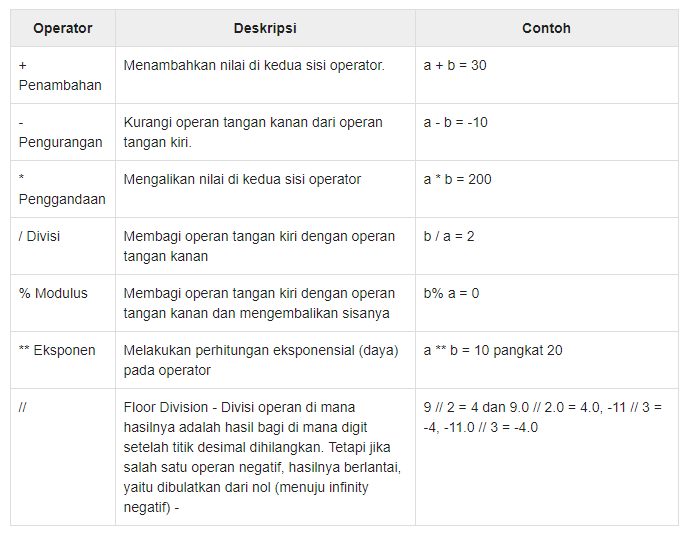
\includegraphics[width=8cm]{figures/xxx.png}
\end{figure}

fungsi  str () untuk mengonversi integer ke String dengan Python\\
penggunaan: \\
m = 2\\
print(str(m))\\

Fungsi  int () adalah fungsi  bawaan standar Python untuk mengubah string menjadi nilai integer.\\
penggunaan\\
m = "2"\\
print(int(m))\\

\section{Looping}
Perulangan For in\\
Perulangan terjadi sampai looping mencapai elemen atau anggota terakhir dari sequence. Bila loop sudah sampai ke elemen terakhir dari sequence, maka program akan keluar dari looping.\\

Perulangan While\\
Perulangan menggunakan while akan menjalankan blok pernyataan terus menerus selama kondisi bernilai benar.//

\section{Kondisi/If Else}
ada 3 kondisi di pyhton. yaitu if, if..else, if..elif..else\\

contoh if\\
umur = 20\\
if umur > 18:\\
    print "Sudah beranjak dewasa"\\

contoh if..else\\
umur = 20\\
if umur > 18:\\
    print "Sudah beranjak dewasa"\\
else:\\
    print "Masih dibawah umur"\\
    
contoh if..elif..else\\
umur = 37\\
if umur > 18 and umur < 30:\\
    print "Sudah beranjak dewasa"\\
elif umur > 30 and umur < 45:\\
    print "Masa - masa emas"\\
elif umur > 45 and umur < 55:\\
    print "Memasuki masa paruh baya"\\
elif umur > 55:\\
    print "Masa - masa manula"\\
else:\\
    print "Masih dibawah umur"\\

\section{Jenis Error yang sering ditemui}

1. Syntax Error\\

       perbaiki perintah atau statement yang diketik.\\
       perbaiki aturan pengkodean.\\

2. Run-time Error\\
      
       cek kembali nama file yang hendak dimasukan.\\
 

\section{Penggunaan Try Except}

a = 12 \\
s = "hello" \\
try: \\
    print("inside try") \\
    print(a + s) \\ 
    print("Printed using original data types") \\
except TypeError: \\
    print("inside except") \\
    print(str(a) + s) \\
    print("Printed using type-casted data types") \\